{\small
\section{Exceptions, Errors}
    \begin{tabular}{l l}
        \tikz[baseline=(text.base)]\node[fill=orange, fill opacity=0.2, text opacity=1, rounded corners, inner sep=2pt, minimum height=5pt] (text) {Errors:};&$\bullet$ Schwerwiegende Fehler, \textbf{nicht behandeln!} \\
        &$\bullet$ Fehler in JVM: OutOfMemoryError, ... \\
        &$\bullet$ Programmierfehler: AssertionError \\
        \hline
        \tikz[baseline=(text.base)]\node[fill=red, fill opacity=0.2, text opacity=1, rounded corners, inner sep=2pt, minimum height=5pt] (text) {Exceptions:};&$\bullet$ Laufzeitfehler, die \textbf{behandelbar} sind \\
        &$\bullet$ fehlerhafte Bedienung, Parameter, ... \\
        &$\bullet$ siehe auch Checked / Unchecked \ref{checked,unchecked} \\
    \end{tabular}
    \vspace{-0.3cm} 

    \subsubsection{Checked, Unchecked}\label{checked,unchecked}
        \begin{tabular}{l}
            \rowcolor[RGB]{239,239,239} 
            \textbf{Checked}\\
            $\bullet$ Exception muss behandelt werden ODER\\
            $\bullet$ \verb|throws|-Deklaration im Methodenkopf\\
            $\bullet$ Wird vom Compiler geprüft\\
            \hline
            \rowcolor[RGB]{239,239,239} 
            \textbf{Unchecked}\\
            $\bullet$ Kein \verb|throws| oder Behandlung nötig\\
            $\bullet$ \tikz[baseline=(text.base)]\node[fill=red, fill opacity=0.2, text opacity=1, rounded corners, inner sep=2pt, minimum height=5pt] (text) {\verb|RuntimeException|}; und \tikz[baseline=(text.base)]\node[fill=orange, fill opacity=0.2, text opacity=1, rounded corners, inner sep=2pt, minimum height=5pt] (text) {Error};, sowie ihre Unterklassen\\
            $\bullet$ Wird nicht vom Compiler geprüft\\
        \end{tabular}
    \vspace{-0.3cm} 

\subsection{Exception auslösen}
    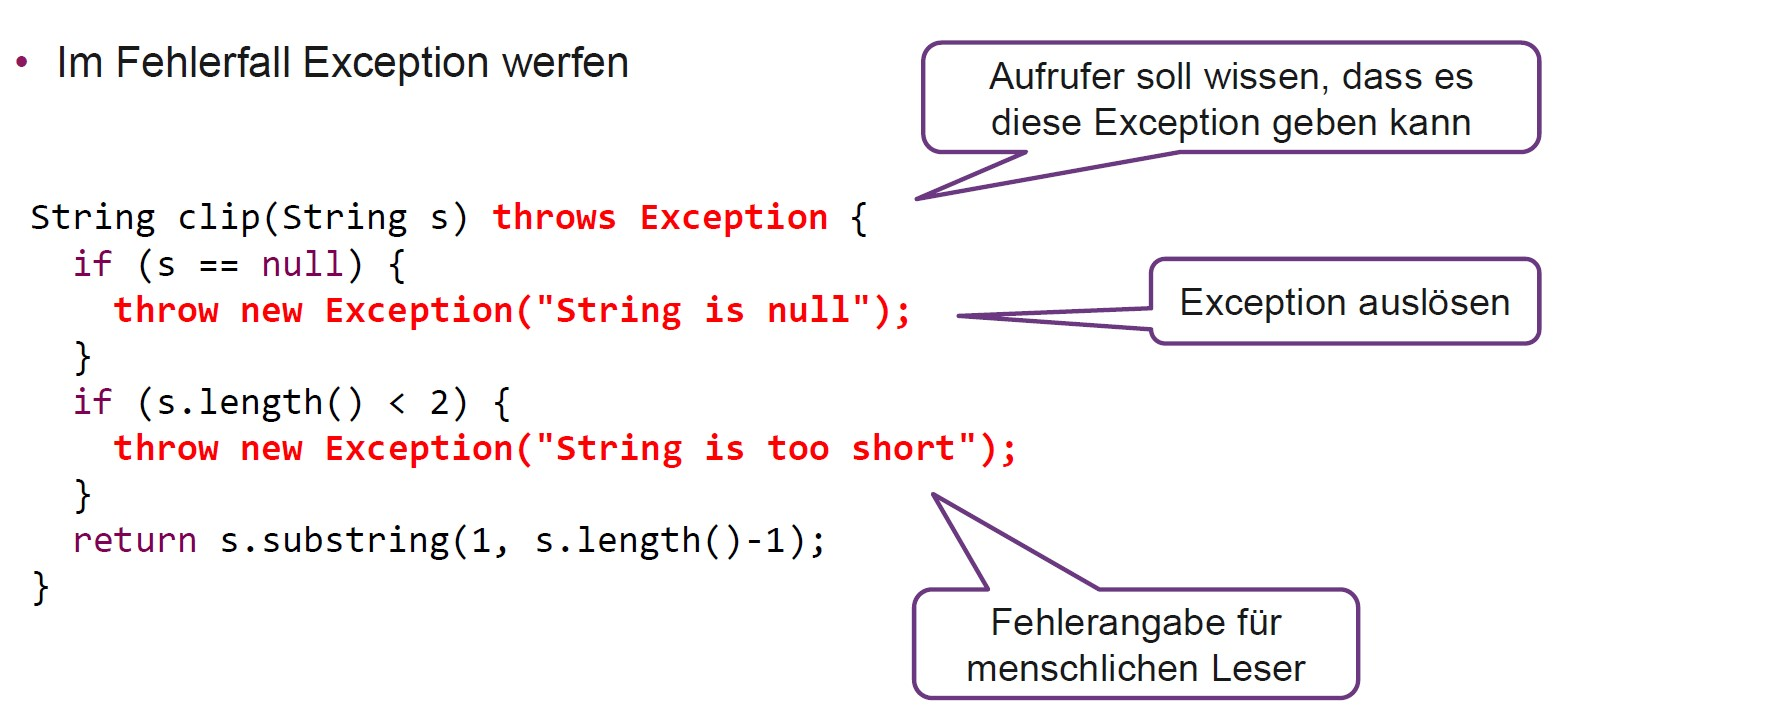
\includegraphics[width=0.85\linewidth]{pictures/exception-throw.jpg}
    \vspace{-0.3cm}

    \subsubsection{throws-Deklaration}
        \begin{tabular}{l}
            $\bullet$ Methode muss alle potentiellen Exceptions deklarieren,\\
            $\qquad$ die der Aufrufer erhalten könnte. (Ausser Unchecked \ref{checked,unchecked})\\
            $\bullet$ Aufrufer muss die Exception behandeln (fangen) / weiterreichen.\\
        \end{tabular}
        \vspace{-0.3cm}

\subsection{Exception behandeln}
    \begin{minipage}{0.7\columnwidth}
        \begin{tabular}{l}
            $\bullet$ Regulärer Code (\verb|try-Block|)\\
            $\bullet$ Fehlerbehandlung (\verb|catch|-Block)\\
                $\qquad\bullet$ Exception im\\
                $\qquad\qquad$ \verb|try-Block| $\rightarrow$ \verb|catch|-Block\\
                $\qquad\bullet$ Keine Exception: \verb|catch|-Block wird\\
                $\qquad\qquad$ nicht ausgeführt\\
            $\bullet$ Opt. \verb|finally|-Block: Wird immer\\
                $\qquad$ durchlaufen\\
        \end{tabular}
    \end{minipage}
    \hfill
    \begin{minipage}{0.35\columnwidth}
        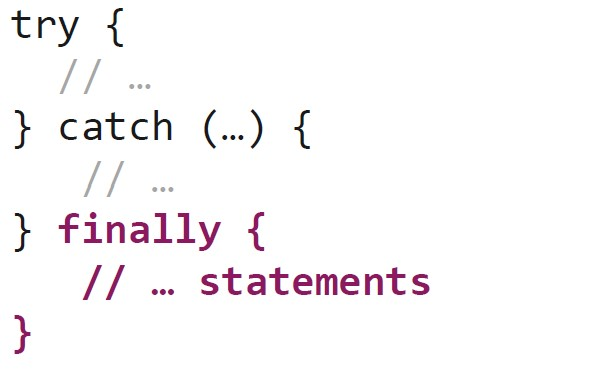
\includegraphics[width=\linewidth]{pictures/try-catch-finally.jpg}
    \end{minipage}

    \begin{tabular}{l}
        \hline
        $\bullet$ Mehrere \verb|catch|-Blöcke: \textbf{Nur} der erste Passende\\
        $\qquad$ (von oben nach unten gesucht) ausgeführt.\\\hline
        $\bullet$ Falls Exception nicht behandelt wird $\rightarrow$ wird die Exception\\
        $\qquad$ zum nächsthöheren Aufrufer geschickt.\\
        $\bullet$ Wenn dies \verb|main()| ist, wird die Exception an die JVM geworfen\\
        $\qquad$ und das Programm abgebrochen.\\  
    \end{tabular}
    \vspace{-0.3cm}

    \subsubsection{try-with-resources $\rightarrow$ für Obj. die geschlossen werden müssen}
        (Interface \verb|AutoCloseable|)\\
        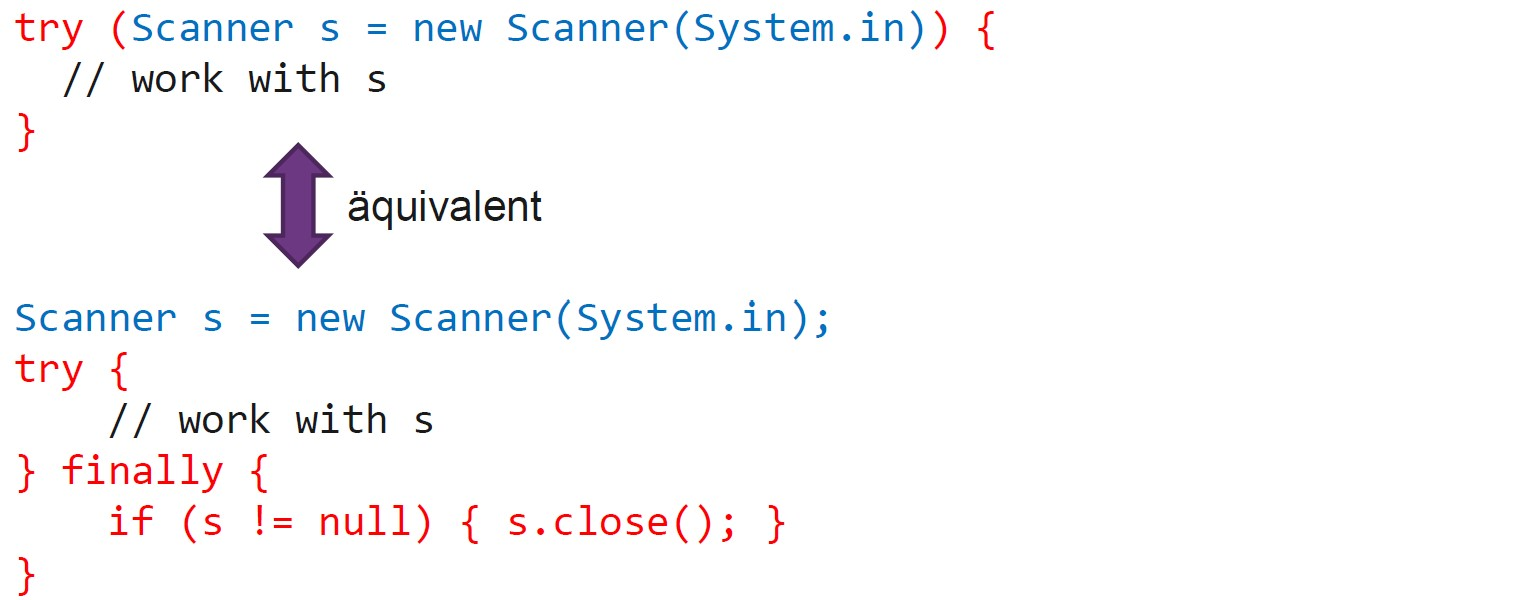
\includegraphics[width=0.85\linewidth]{pictures/try-with-resources.jpg}
        \vspace{-0.2cm}
}